\documentclass[whitelogo]{tudelft-report}
\usepackage{natbib}
\usepackage{changes}

%% to compile the pdf do:
%% xelatex report
%% bibtex report
%% xelatex report
%% xelatex report


\begin{document}

%% Use Roman numerals for the page numbers of the title pages and table of
%% contents.
\frontmatter

%% Uncomment following 19 lines for a cover with a picture on the lower half only
%\title[tudelft-white]{Title}
%\subtitle[tudelft-cyan]{Optional subtitle}
%\author[tudelft-white]{J.\ Random Author}
%\affiliation{Technische Universiteit Delft}
%\coverimage{cover.jpg}
%\titleoffsetx{10cm}
%\titleoffsety{10cm}
%\afiloffsetx{1cm}
%\afiloffsety{18cm}
%\covertext[tudelft-white]{
%    \textbf{Cover Text} \\
%    possibly \\
%    spanning 
%    multiple 
%    lines
%    \vfill
%    ISBN 000-00-0000-000-0
%}
%\makecover

%% Uncomment following 16 lines for a cover with a picture on the lower half only
\title[tudelft-white]{CIE5308}
\subtitle[tudelft-black]{Assignment}
\author[tudelft-white]{{J. Gundlach} -- {C. Rozas} -- {L. Lange}}
\affiliation{Delft University of Technology}
\coverimage{title.jpg}
\covertext[tudelft-white]{
    \textbf{Group 3} \\
    %possibly \\
    %spanning 
    %multiple 
    %lines
    \vfill
}
\setpagecolor{tudelft-cyan}
\makecover[split]


%% Include an optional title page.
\begin{titlepage}


\begin{center}

%% Insert the TU Delft logo at the bottom of the page.

%% Print the title in cyan.
{\makeatletter
\largetitlestyle\fontsize{64}{94}\selectfont\@title
%\largetitlestyle\color{tudelft-cyan}\Huge\@title
\makeatother}

%% Print the optional subtitle in black.
{\makeatletter
\ifx\@subtitle\undefined\else
    \bigskip
   {\tudsffamily\fontsize{22}{32}\selectfont\@subtitle}    
    %\titlefont\titleshape\LARGE\@subtitle
\fi
\makeatother}

\bigskip
\bigskip

by
%door

\bigskip
\bigskip

%% Print the name of the author.
{\makeatletter
%\largetitlefont\Large\bfseries\@author
\titlestyle\fontsize{10}{10}\selectfont\@author
\makeatother}

\bigskip
\bigskip

% to obtain the degree of Master of Science
% %ter verkrijging van de graad van Master of Science
% 
% at the Delft University of Technology,
% %aan de Technische Universiteit Delft,
% 
% to be defended publicly on Tuesday January 1, 2013 at 10:00 AM.
% %in het openbaar de verdedigen op dinsdag 1 januari om 10:00 uur.

\vfill

\begin{tabular}{lll}
    Student numbers: & 4450426 -- 4519388 -- 4512022 \\
    Project duration: & \multicolumn{2}{l}{March 17, 2016 -- April 1, 2016} \\
%     Thesis committee: & Prof.\ dr.\ ir.\ J.\ Doe, & TU Delft, supervisor \\
%         & Dr.\ E.\ L.\ Brown, & TU Delft \\
%         & Ir.\ A.\ Aaronson, & Acme Corporation
\end{tabular}
%% Only include the following lines if confidentiality is applicable.

% \bigskip
% \bigskip
% \emph{This thesis is confidential and cannot be made public until December 31, 2013.}
% %\emph{Op dit verslag is geheimhouding van toepassing tot en met 31 december 2013.}

% \bigskip
% \bigskip
% An electronic version of this thesis is available at \url{http://repository.tudelft.nl/}.
% %\\[1cm]

%\centering{
\includegraphics{cover/logo_black}}


\end{center}

\begin{tikzpicture}[remember picture, overlay]
    \node at (current page.south)[anchor=south,inner sep=0pt]{
        
\includegraphics{cover/logo_black}
    };
\end{tikzpicture}

\end{titlepage}



% \chapter*{Preface}
\setheader{Preface}

Preface\ldots

\begin{flushright}
{\makeatletter\itshape
    \@author \\
    Delft, January 2013
\makeatother}
\end{flushright}



\tableofcontents

%% Use Arabic numerals for the page numbers of the chapters.
\mainmatter

\chapter{Notes}

\section{18.03.16 - lecture introducing exercise}

\textbf{Main aim}: design breakwater
\begin{enumerate}
 \item new breakwater
 \item adjust existing one
\end{enumerate}

\textbf{Location}:
\begin{itemize}
 \item ..
\end{itemize}

\textbf{Present situation}:
\begin{itemize}
 \item cross-section, what they were supposed to build
 \item slide 9: measured cross-section
\end{itemize}

\textbf{Assignment}:
\begin{itemize}
 \item three locations
 \item three design lifes: after so many years needs to be maintained/rebuild, not for design cinditions!
 \item something with the existing (Bas)...?
\end{itemize}

\textbf{Design}:
\begin{itemize}
 \item assume: subsoil no problem
 \item Any idea where the rock comes from? Quarries in ALbania? Albania exports a lot of Marble to Italy. How about the stones sorted out?
 \item Infra structure in Albania not as good.
 \item Google Earth because you can check time. Check -design period and +design period from present.
 \item Play with colors in picture editor. Image processing for bathymetry stuff.
 \item Map Room: Libarary of faculty of architecture, first floor within library. And webpage of this library? And webapp.navionics.com (not working for 4G.
 \item Check wave data from design wind speed $\rightarrow$ should be in same magnitude as from Argoss (verify data)
\end{itemize}

\textbf{Argoss}:
\begin{itemize}
 \item sells  wave data
 \item www.waveclimate.com
 \item TuDelft DuT4321 valid until 31.3.
 \item Size of piece: find balance (density of data is the same, too big, not appropriate anymore, too small, not enough data any more)
 \item 1D, 2D, 3D
 \item don't use their model for nearshore
\end{itemize}

\textbf{B.C.}:
\begin{itemize}
 \item B.C. damage vs. B.C. operation of port
 \item 
\end{itemize}

\textbf{Presentation}:
\begin{itemize}
 \item Why did you make this choices you made?
 \item Presentation and questions of group will be graded.
 \item No obvious information in the presentation
 \item 
\end{itemize}

\textbf{Report}:
\begin{itemize}
 \item Indicate 2.1 to 2.6 clearly in report
 \item Make it possible to enable contractor for a pricing
 \item Drawing on A3
 \item only cross-section, only one
 \item head needs not to be designed?
 \item only 10 pages text
 \item report should be understandable without annex
 \item 
\end{itemize}

\textbf{Calculation}:
\begin{itemize}
 \item bonus for differences due classical and probabilistic approach
 \item No assessment on skills in maths
 \item 
\end{itemize}

\textbf{PIANC}:
\begin{itemize}
 \item kennisbank waterbouw
 \item ''codes, standards and design guides``
 \item ...
 \item ''Books and reports``
\end{itemize}


\textbf{Check}:
\begin{enumerate}
 \item google earth
 \item make pdfs from ppt's
 \item Argoss book online or from library
 \item check demands on slides, slide 21  e.g.
 \item 
\end{enumerate}



\chapter{Introduction}

\section{General Task}

By \textit{Group 3} the breakwater in the South is looked at:
\begin{itemize}
 \item adjacent to roundhead, axis 315\textsuperscript{o}
 \item rubble mound single layer cubes
 \item rehabilitation
 \item 100 years design life
 \item quay wall in future
\end{itemize}

\citep{Geim2001} $\leftarrow$ this can be deleted as soon, as there is any other citation we can place, so to prevent error messages due to ``no citations found''

%% Use letters for the chapter numbers of the appendices.
\appendix

\chapter{Function GumbelUnc.mat}


\begin{figure}[H]
\center
\fbox{
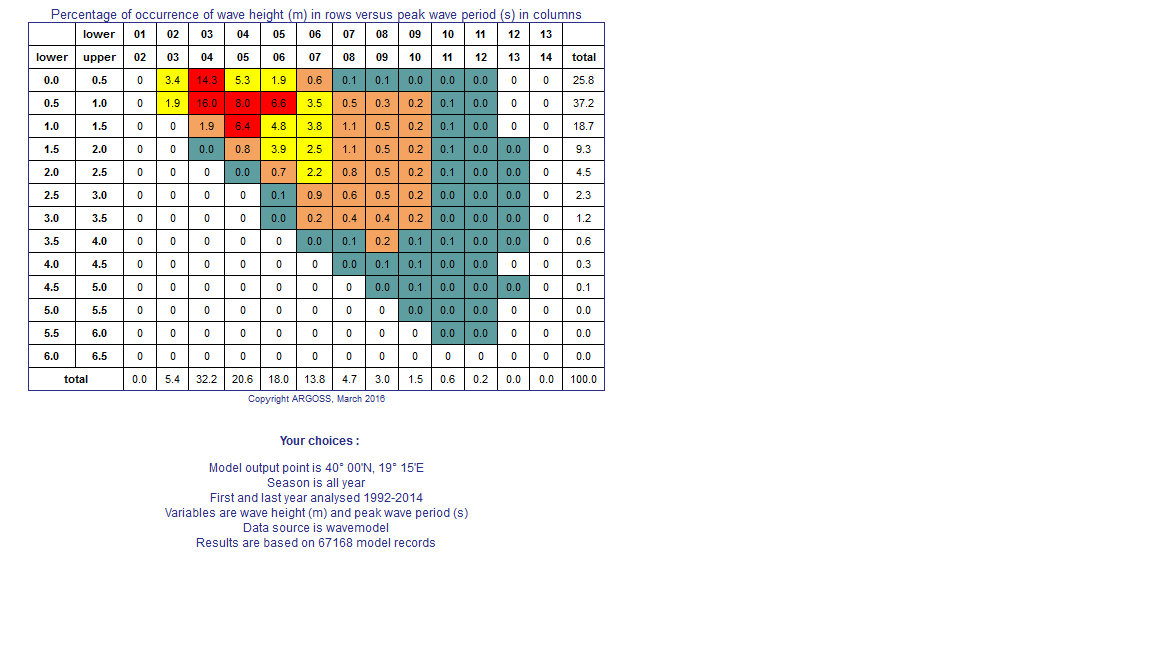
\includegraphics[width=\textwidth]{images/wave_pperiod_allyear.png} 
}
\caption[Distribution of peak-period over wave hight]{Distribution of peak-period over wave hight}
%\label{Distribution_pperiod}
\end{figure}


\begin{figure}[H]
\center
\fbox{
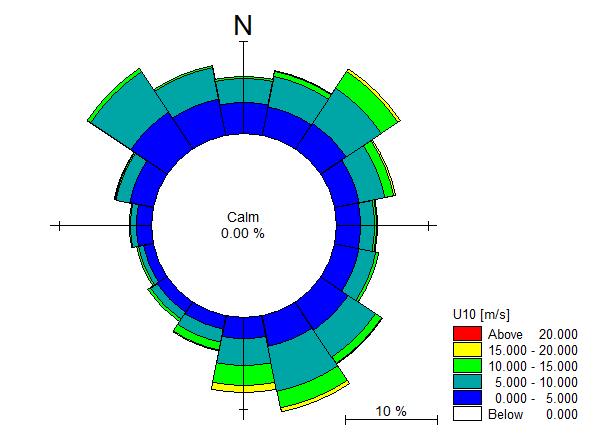
\includegraphics[width=\textwidth]{images/Rose_plot_u10.png} 
}
\caption[Rose-diagram with the distribution of the wind}
%\label{Windrose}
\end{figure}


\begin{figure}[H]
\center
\fbox{
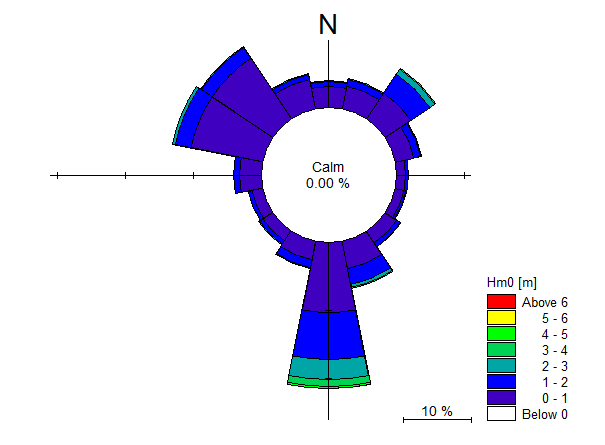
\includegraphics[width=\textwidth]{images/Rose_plot_Hoverall.png} 
}
\caption[Rose-diagram with the distribution of the waves}
%\label{wavedata_angle}
\end{figure}
Whatever XX


\bibliography{report}

\end{document}

